% This is samplepaper.tex, a sample chapter demonstrating the
% LLNCS macro package for Springer Computer Science proceedings;
% Version 2.20 of 2017/10/04
%
\documentclass[runningheads]{llncs}
%
\usepackage{bbding}
\usepackage{graphicx}
\usepackage{cite}
\usepackage{amsmath,amssymb,amsfonts}
%\usepackage{algorithmic}
\usepackage{textcomp}
\usepackage{xcolor}
\usepackage{algorithm}
\usepackage{algpseudocode}
\usepackage{amsmath}
\usepackage{graphics}
\usepackage{epsfig}
\usepackage{booktabs}
% Used for displaying a sample figure. If possible, figure files should
% be included in EPS format.
%
% If you use the hyperref package, please uncomment the following line
% to display URLs in blue roman font according to Springer's eBook style:
% \renewcommand\UrlFont{\color{blue}\rmfamily}

\begin{document}
%
\title{A Novel Thought of Pruning Algorithms: Pruning Based on Less Training\thanks{Supported by organization x.}}
%
%\titlerunning{Abbreviated paper title}
% If the paper title is too long for the running head, you can set
% an abbreviated paper title here
%
\author{Yue Li\inst{} \and
Weibin Zhao\inst{} \and
Lin Shang\inst{(}\Envelope\inst{)}}
%\orcidID{2222--3333-4444-5555}}...
%
\authorrunning{L. Yue, Z. Weibin et al.}
% First names are abbreviated in the running head.
% If there are more than two authors, 'et al.' is used.
%
\institute{Department of Computer Science and Technology,\\
 Nanjing University, Nanjing 210023, China\\
\email{mf1633021@smail.nju.edu.cn, njzhaowb@gmail.com,\\ shanglin@nju.edu.cn}\\
%\url{http://www.springer.com/gp/computer-science/lncs} \and
%ABC Institute, Rupert-Karls-University Heidelberg, Heidelberg, Germany\\
%\email{mf1633021@smail.nju.edu.cn,njzhaowb@gmail.com,shanglin@nju.edu.cn}
}
%
\maketitle              % typeset the header of the contribution
%
\begin{abstract}
Pre-training of models in pruning algorithms plays an important role in pruning decision-making. We find that excessive pre-training is not necessary for pruning algorithms. According to this idea, we propose a pruning thought---\textbf{Incremental pruning based on less training (IPLT)}. We can combine \textbf{IPLT} with almost all existing pruning algorithms. Compared with the original pruning algorithms based on a large number of pre-training, the modified algorithms (by \textbf{IPLT}) has competitive compression effect. On the premise of ensuring accuracy, the pruning algorithms modified by \textbf{IPLT} can achieve 8x-9x compression for VGG-16 on CIFAR-10 and only needs to pre-train few epochs. For VGG-16 on CIFAR-10, we can not only achieve 10x test acceleration, but also about 10x training acceleration. At present, the research mainly focuses on the compression and acceleration in the application stage of the models, while the compression and acceleration in the training stage are few. We newly proposed the thought of \textbf{IPLT} that can compress and accelerate in the training stage. It is novel to consider the amount of pre-training required by pruning algorithm. Our results have implications: Too much pre-training may be not necessary for pruning algorithms.

\keywords{pruning algorithms \and amount of pre-training \and too many.}
\end{abstract}
%
%
%
\section{Introduction}
Deep neural networks have achieved excellent results in many competitions. The outstanding performance of the deep learning model has attracted the attention of academic and industrial circles. From AlexNet\cite{b1} to VGG-16\cite{b2}, ResNet\cite{b3} and InceptionNet\cite{b4}, it's not hard to see that the superior performance of deep learning models often depends on deeper, wider structures. A deeper deep learning model leads to better recognition accuracy, but it will consume more storage and computation resource. To solve these problems, the researchers proposed a series of model compression and acceleration algorithms.

Most previous works on accelerating CNNs can be roughly divided into three categories, namely, matrix decomposition \cite{b5}, \cite{b6}, quantization \cite{b7}, \cite{b8} and pruning \cite{b9}, \cite{b11}, \cite{b27}, \cite{b28}, \cite{b30}.


\begin{figure}
\centering
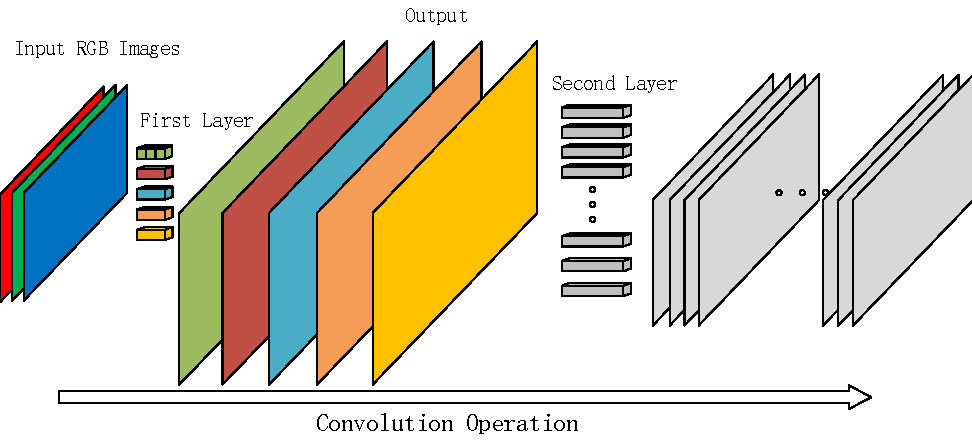
\includegraphics[width=.5\textwidth]{convolution_operation.pdf}
\caption{This picture shows the convolution process of two convolution layers. The convolution network's input is an RGB image. In this picture, each cube in the graph corresponds to a filter. There are five filters in the first layer, so there are five output feature maps in the first layer. We use the same color to show the corresponding relationship between filters and output feature graphs. Notice the first filter in the first layer, which consists of three blocks. In convolution operation, each block corresponds to one input feature map.}
\label{fig:convolution_operation}
\end{figure}

As early as 1990, \cite{b23} began to pruning the neural network. Before 2016, the pruning algorithm mainly focused on pruning the parameters of the models. In \cite{b9}, the author determines the importance of the parameter according to the absolute values of the parameters. The author assume the smaller parameters are less important and will be cut off first. The algorithm mentioned in \cite{b9} is also used by \cite{b10}, which greatly compresses the deep learning model.

Then in 2016 and 2017 years, a large number of papers began to focus on the pruning of the deep learning models' filters. Such as \cite{b19}, \cite{b20}, \cite{b21}, \cite{b22}, these papers began to try to slim down the structure of the model. By pruning the filters of the model, the model can be accelerated without relying on specific libraries. We can see the details of the convolution operation and the role of filters in the convolution operation through Fig.\ref{fig:convolution_operation}.

As shown in the left of the Fig.\ref{fig:pruning_contrast}, almost all pruning algorithms have a general flow of pre-training models, pruning and retraining.  In order to prune better and search for the effective inner structure of the model, the existing pruning algorithms need a long pre-training process for pre-training models , which usually requires hundreds of training epochs. As far as we known, almost all pruning algorithms pruning the models after hundreds of pre-training epochs. In response to this situation, we raised a question: the longer the training, the more effective the pruning decision will be made?

\begin{figure}
\centering
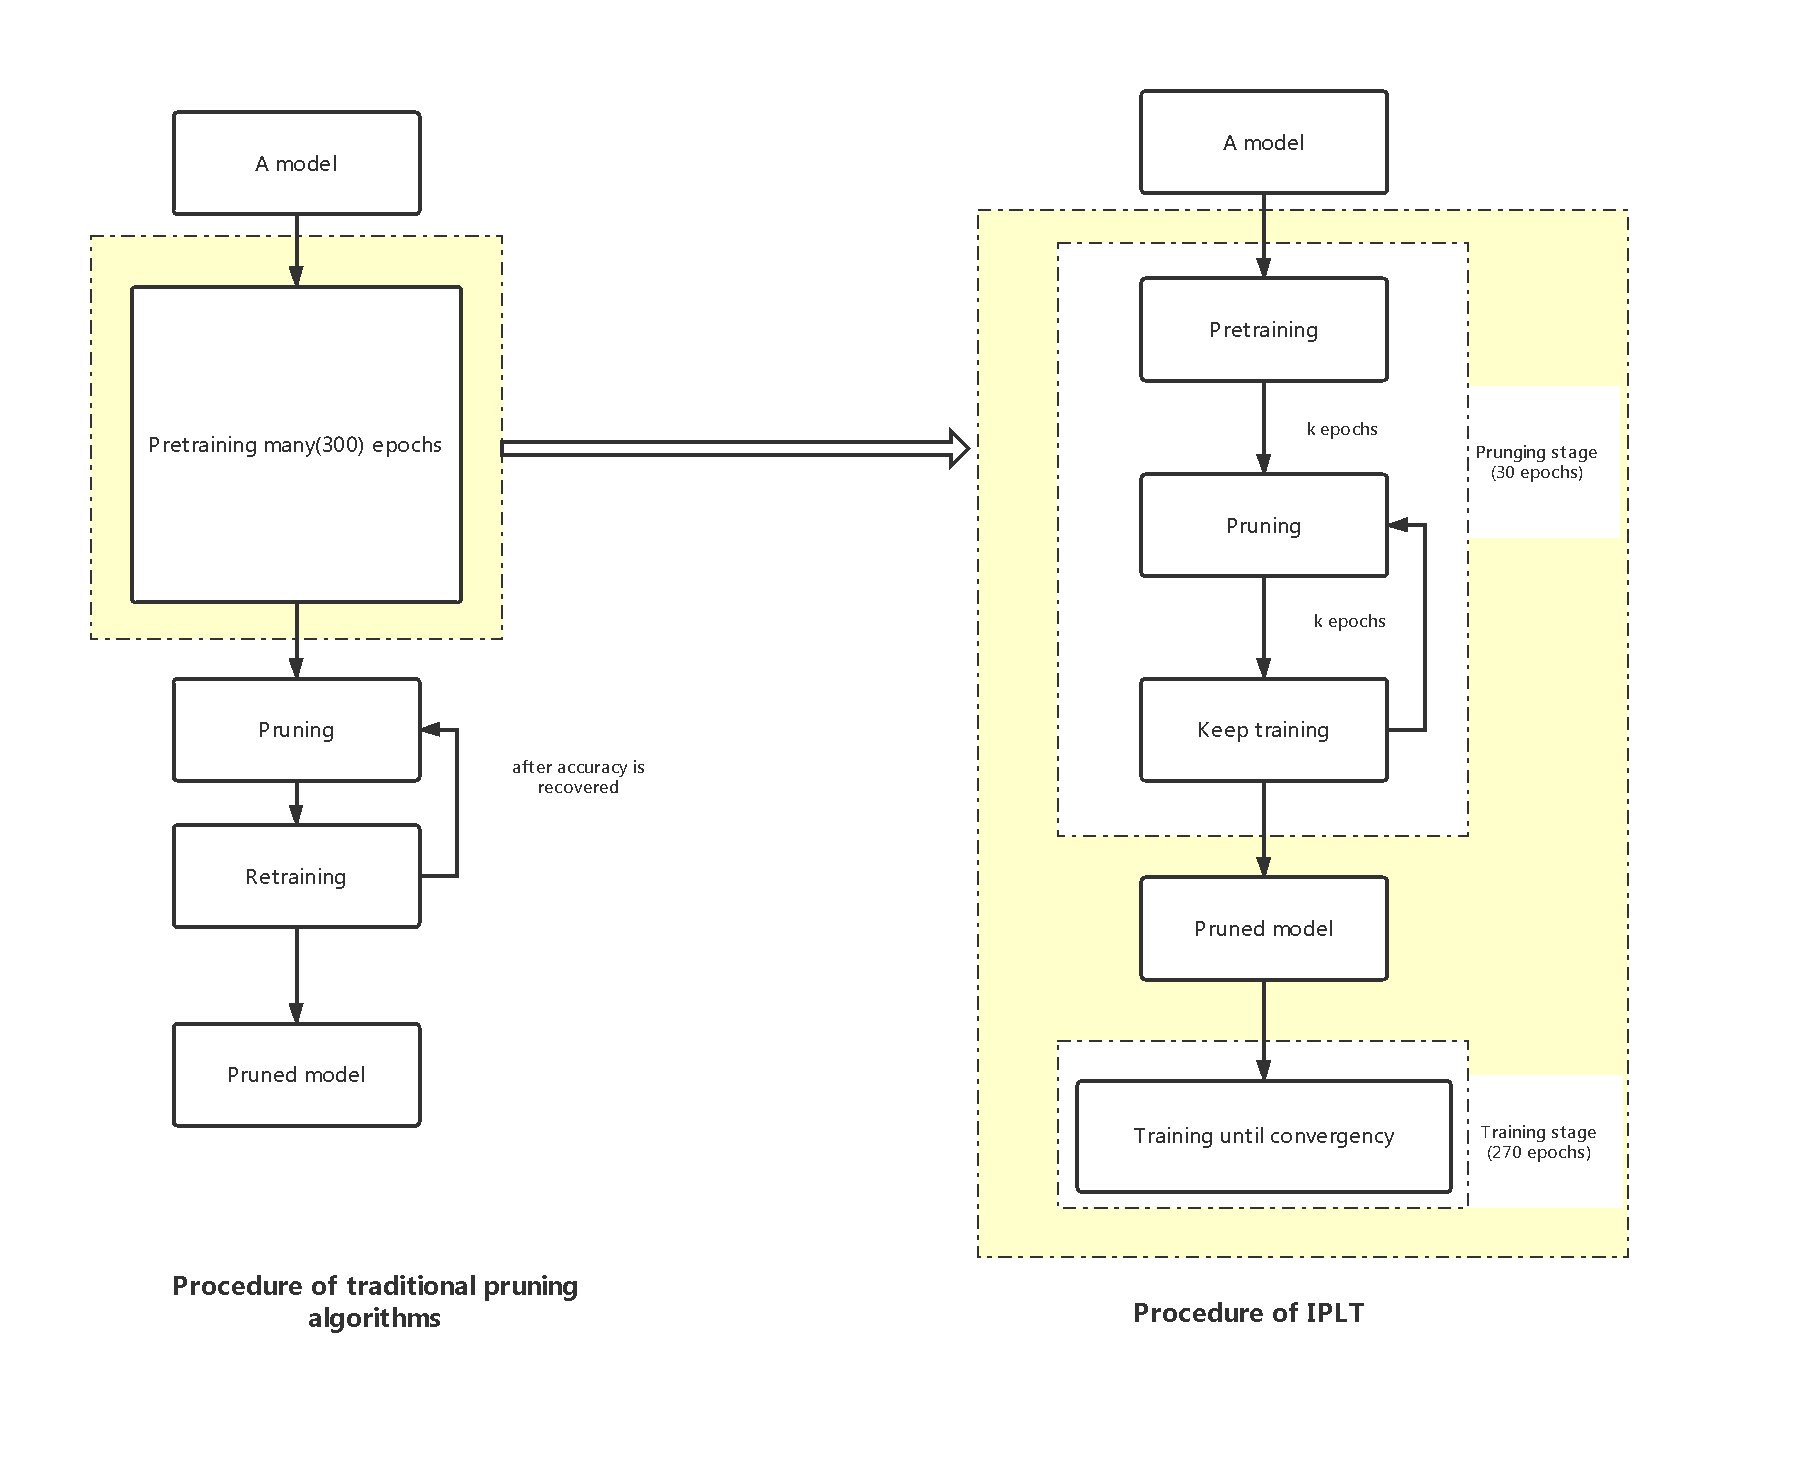
\includegraphics[width=.5\textwidth]{pruning_contrast.pdf}
\caption{In this picture, the general flow of the traditional pruning algorithm is on the left, and the general flow of \textbf{IPLT} is on the right. It is not difficult to find that the biggest feature of \textbf{IPLT} is: first pruning, then training. \textbf{IPLT} only trains few epochs to prune the model, and in the training phase of the model, a lot of computing resources will be reduced.}
\label{fig:pruning_contrast}
\end{figure}

$\textbf{Our Point of View:}$



$\textbf{The Origin of \textbf{IPLT}:}$
We think that the traditional pruning algorithm pays too much attention to the pre-training process. Previous researchers often believed that the longer the pre-training process was, the more effective the pruning strategy was. Of course, if we were allowed to prune the model only once, it would be wise to do more pre-training. But in the actual pruning process, we focus on the model obtained by pruning, and do not limit the number of pruning.  And in many papers, researchers have found that the general iteratively pruning strategy is more effective, that is, the small-step pruning strategy can effectively avoid pruning excessive damage to the effective structure of the model. Therefore, there is a question worth thinking about: if we only prune a small part of the parameters or filters at a time, do we need a lot of pre-training or even training the model to convergence before the first pruning operation? We believe that a small amount of pre-training is enough to complete a small-step pruning on deep learning model. Based on this idea, we propose the thought of \textbf{Incremental Pruning Based on Less Training(IPLT)}. In contrast, we can call the thought behind all existing pruning algorithms \textbf{Pruning Based on Much Training(PMT)}



$\textbf{Rough Flow of \textbf{IPLT}}$
We can use the thought of \textbf{IPLT} to improve almost all existing pruning algorithms.
The comparison between \textbf{IPLT} and traditional pruning thought(\textbf{PMT}) is placed on Fig.\ref{fig:pruning_contrast}. The biggest difference between \textbf{IPLT} and \textbf{PMT} is that the model is pruned first and then trained to convergence. As shown in the figure, on the right, \textbf{IPLT} is roughly divided into pruning and training stages.\\
\textbf{Pruning Stage} \quad we need to set the hyperparameter $k$. Every time we train $k$ epoches continuously, we prune the network once. When we do the pruning operation, we can utilize any criterion in existing pruning algorithms. Assuming $k=5$, our ultimate goal is to prune $90\%$ of a layer of network. The pruning ratio list is $[10\%,20\%,30\%, \dots,90\%]$. We can prune $10\%$ of all filters in network's convolution layer for the first time. At the second pruning, another $10\%$ filters are pruned, the percentage of pruning reaches $20\%$. Every pruning operation, $10\%$ extra filters are pruned until $90\%$ of filters are pruned. \\
\textbf{Training Stage} \quad When pruning reaches the target pruning ratio, we stop pruning, but keep training the pruned network until convergence.
By pruning the model step by step, our method achieves the ideal pruning ratio, and avoids the excessive pruning of the model at one time, which affects the performance.

To verify the feasibility of the thought \textbf{IPLT}, We utilize our \textbf{IPLT} idea to implement two existing pruning algorithms \cite{b35}, \cite{b27}. By the contrast experiments, we find the pruning performance of the two modified pruning algorithms is not weaker than original algorithms(\textbf{PMT}). For simplicity of expression, we will sometimes use \textbf{IPLT} to represent the pruning algorithms modified by the thought of \textbf{IPLT}.  \textbf{PMT} will sometimes be used to represent original pruning algorithms.

$\textbf{The Uniqueness and Contribution of Our Work:}$\\
1.  Proposing a novel thought \textbf{IPLT}. As far as we known, \textbf{IPLT} is the first to consider number of pre-training epochs before pruning decision. This thought is different from the thought behind any existing pruning algorithms(\textbf{PMT}) and has been proved effective;\\
2. As far as we know, the two pruning algorithms modified by \textbf{IPLT} in this paper are the first two pruning algorithms to optimize the computational complexity during model's pre-training stage. As shown in right of Fig.\ref{fig:pruning_contrast}, assuming that we train 300 epochs for the model, the pruning algorithm based on IPLT will finish pruning the model in the first 20 to 40 epochs, and then train the smaller model. Obviously, in 41th to 300th epoch, we train the pruned ,small models (the traditional algorithm trains the original model, big). In forward propagation and back propagation, smaller models consume less computing resources naturally. Therefore, \textbf{IPLT} make the training of models consuming much less computation resources as original.\\


\section{Related Works}
Our algorithm is about pruning. At present, pruning algorithms can be divided into two categories: weight pruning and filters pruning. We classify pruning related content as follows:
\subsection{Weights Pruning}
Many researchers try to construct sparse convolution kernels by pruning the weight of the network, so as to optimize the storage space occupied by the model. As early as around 1990, both \cite{b15} and \cite{b23} pruned the network parameters based on the second-order derivative, but this method has a high computational complexity.  In \cite{b12}, \cite{b16}, the author regularize neural network parameters by group Lasso penalty leading to sparsity on a group level. In \cite{b9}, the author judges the importance of parameters according to their value, and then prune the unimportant parameters. The \cite{b10} combine the methods in \cite{b9} with quantization, Huffman encoding, and achieve maximum compression of CNNs. \cite{b14} regularize neural network parameters by
group Lasso penalty leading to sparsity on a group level. In order to prevent overpruning, \cite{b11} proposed a parameter recovery mechanism.
By pruning the parameters, a sparse model can be constructed. This kind of method can compress the model storage. Because the application of these pruned models always depend on specific libraries, computational optimization is not sufficient. So in the past two years, many researchers have turned their attention to pruning filters.

\subsection{Filters Pruning}
In the past two years, there has been a lot of work about filters pruning algorithms. Most papers use certain criteria to evaluate filters, and ultimately prune unimportant filters. In 2017, \cite{b17}  try to use $l1-norm$ to select unimportant filters. \cite{b18} uses the scaling factor $\gamma$ in batch normalization as an important factor, that is, the smaller the $\gamma$ is, the less important the corresponding channel is, so that filters can be pruned. \cite{b21} proposes a Taylor expansion based pruning criterion to approximate the change in the cost function induced by pruning.
In addition to pruning filters through specific criteria, some researchers also proposed new ideas. \cite{b28} proposed utilizing a long short-term memory (LSTM) to learn the hierarchical characteristics of a network and generate a pruning decision for each layer. \cite{b29} proposed a model pruning technique that focuses on simplifying the computation graph of a deep CNN. In \cite{b27}, the author proposed a Soft Filter Pruning (SFP) method to accelerate the inference procedure of deep CNNs.

In addition to the above papers, some researchers \cite{b12}, \cite{b13} have proposed algorithms that can be used to prune both parameters and filters.


\section{Methodology}
\subsection{Preliminaries}\label{AA}
In this section, we will formally introduce the symbol and annotations. We use $\left\{\mathcal{W}_i \in \mathbb{R}^{O_i \times I_i \times K \times K} , 1\leq i \leq L \right\}$ and $\left\{b_i \in \mathbb{R}^{O_i} , 1\leq i \leq L \right\}$to denote ith convolutional layer's weights and bias, L is the number of layers. $\textbf{I}_i$ and $\textbf{O}_i$ denote the number of input and output feature maps in ith layer, so the input tensor of $i-th$ layer can be represented by $\textbf{FI}_i$ and its size is $I_i \times H_i \times \mathcal{W}_i$, output tensor of $i-th$ layer can be represented by $\textbf{FO}_i$ and its size is $O_i \times H_{i+1} \times \mathcal{W}_{i+1}$. Obviously, $\textbf{FI}_(i+1) = \textbf{FO}_i$, and in CNNs with RGB images $\textbf{I}_1 = 3$. $\mathcal{F}_{i,j}$ represent $j-th$ filter in CNNs' $i-th$ layer, $\mathcal{F}_{i,j} \in \mathbb{R}^{I_i \times K \times K}$. The convolutional operation of $i-th$ layer can be written as:

\begin{equation}
FO_{i} = \mathcal{W}_i \ast FI_i + b_i, 1\leq i \leq L
\label{equ.1}
\end{equation}

Equation.\ref{equ.2} can be seen as a composite of  $O_i$ filters' convolutional operation:

\begin{equation}
FO_{i,j} = \mathcal{F}_{i,j} \ast FI_i, 1\leq j \leq O_i
\label{equ.2}
\end{equation}

where $FO_{i,j}$ is the $jth$ output feature map of $i-th$ layer. Obviously, $FO_{i} = \left\{FO_{i,j},  1\leq j \leq O_i \right\}$.

We use $R_i$ to indicate the percentage of filters pruned from $i-th$ Layer to all filters in the same layer. In this case, the number of filters and output feature maps in $i-th$ layer will be reduced to $(1-R_i)O_i$, so the parameters of $i-th$ layer will be reduced from $O_i \times I_i \times K \times K$ to $(1-R_i)O_i \times I_i \times K \times K$. Not only the $i-th$ layer's filters pruned but also the $(i+1)-th$ layer will be affected. As shown in \ref{fig:filters_pruning}, the filters in the $i-th$ layer are pruned, so in the next layer, each filter should be slimmed down. $\mathcal{F}_{i+1,j} \in \mathbb{R}^{O_i \times K \times K}$ should be transformed into $\mathcal{F}^{'}_{i+1,j} \in \mathbb{R}^{(1-R_i)O_i \times K \times K}$


\subsection{How to Select Filters}
In the two papers which we choose to make comparison tests, both the authors choose $\emph{l}_p-$norm of filters to measure the importance of each filter as Eq.\ref{norm}. So we choose the same criterion.
\begin{equation}
    \|\mathcal{F}_{i,j}\|_p = \sqrt[p]{\sum_{n=1}^{I_i} \sum_{k_1=1}^K \sum_{k_2=1}^K |\mathcal{F}_{i,j}(n,k_1,k_2)|^p}
\label{norm}
\end{equation}
In their papers, filters with smaller $\emph{l}_2-$norm result in relatively small activation values, so they think these filters are even less important to the model. The filters with smaller $\emph{l}_p-$norm will be pruned firstly. When we compare the $\emph{l}_p-$norm of filters, we can choose either intra-layer comparison (intra-layer mode) or full-network comparison (global mode). The only difference between intra-layer comparison and full-network comparison is whether all filters in the whole network are sorted together (full-network comparison) or within each layer (intra-layer comparison) when filters are sorted in norm value. We show the general procedure of \textbf{IPLT} in Alg.\ref{alg:global}.

%\begin{figure}
%\centering
%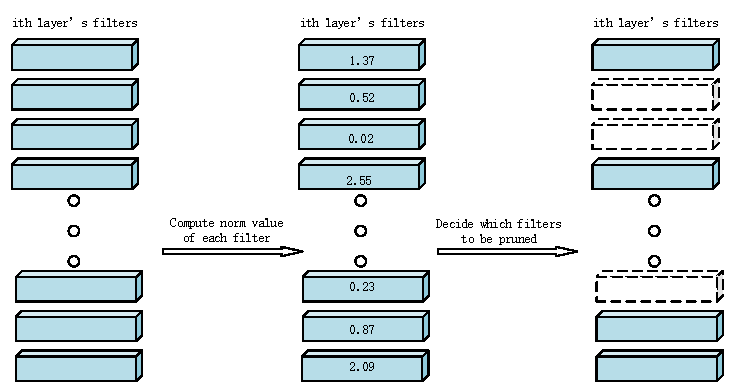
\includegraphics[width=.5\textwidth]{select_filters_to_prune.pdf}
%\caption{This picture shows a pruning operation. We calculate the $\emph{l}_2-$norm of filters in $i-th$ layer, and prune filters with smaller norm by sorting. The first column is all filters in $i-th$ layer. The second column shows that we have calculated the norm values corresponding to each filter in $i-th$ layer. The filters drawn by dashed lines in the third column are pruned. Obviously, filters with smaller norm values are more pruned first. This figure only shows the importance comparison of filters in intra-layer mode; if it is global comparison mode, then we will sort the norm values of filters in all convolution layers and prune filters with small norm values. }
%\label{fig:select_filters_to_prune}
%\end{figure}


\begin{algorithm}[htb]
  \caption{Pruning algorithms modified by \textbf{IPLT}}
  \label{alg:global}
  \begin{algorithmic}[1]
    \Require
      training data:X, training epoches: $epoch_{max}$,
      incremental pruning sequence: $L = \left\{R_1, R_2, ..., R_n\right\}$ ,
      model parametes: $\mathcal{W} = \left\{\mathcal{W}_i , 1\leq i \leq L \right\}$,
      A CNN model, ${W_l,1\leq l\leq L}$;\\
    \Ensure
      Parameters in L layers of the model:${\hat{W_l}, 1\leq l\leq L}$;
    \State Initial: ${W_l}$, ${1\leq l\leq L}$ ; hyper-paramter: k;ind=0;
    \label{code:fram:extract}
    \State for ${epoch=1, 2, \ldots, epoch_{max}}$, do;
    \label{code:fram:trainbase}
    \State \qquad if epoch\%k==0:
    \label{code:fram:add}
    \State \qquad \qquad for $i=0, 1\leq i\leq L$, do:
    \label{code:fram:classify}
    \State \qquad \qquad \qquad Calculate the importance for each filter $\mathcal{F}_{i,j}, 1\leq j \leq I_i$ according to certain criterion;
    \label{code:fram:select} \\
    \State \qquad \qquad  Prune $R_{ind}\ast\sum_{i=1}^LO_i$ filters with minmum importance value in all layers(global) or per layer(intra-layer);
    \State \qquad \qquad ind = ind+1
    \label{code:fram:classify}
    \State \qquad Update model parameters $W$ based on $X$;
    \label{code:fram:add}
    \label{code:fram:select}
    \State Return a pruned and trained model which can be applied directly;
  \end{algorithmic}
\end{algorithm}

Experiments show that globally sorting filter norms and pruning filters can better guarantee network performance.

\subsection{The thought of incremental pruning}
Even based on much pre-training, pruning models to targeted ratio within one pruning operation will also have impacts on the accuracy of the model. So we introduce the thought of incremental. For example, according to the sequence $[10\%, 20\%, 30\%, 40\%, 50\%, 60\%, 70\%]$, we will first cut 10\% of the filters, then cut off the extra 10\% (achieve 20\% pruning rate). By gradually pruning, we keep pruning a small number of filters which are not important, and finally achieve the desired pruning ratio.


\subsection{Details of Pruning Filters}

In Fig.\ref{fig:filters_pruning}, we show the operations performed when pruning a layer.

\begin{figure}
\centering
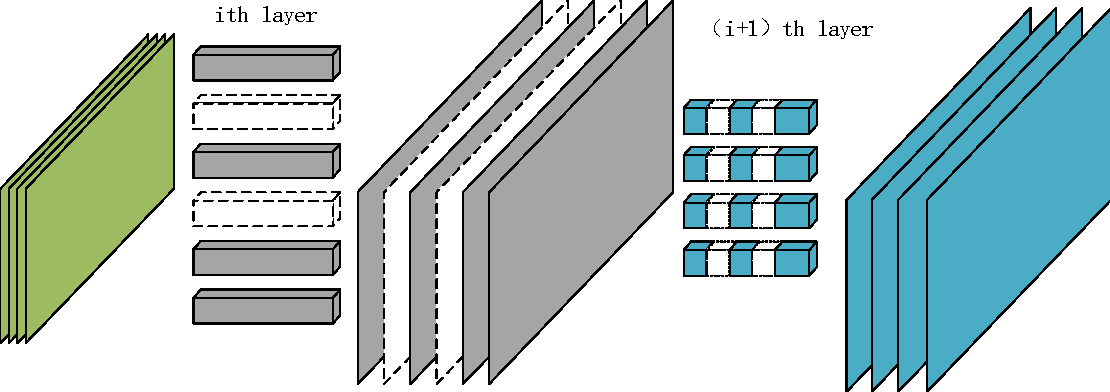
\includegraphics[width=.5\textwidth]{filters_pruning.pdf}
\caption{This picture shows that when we prune filters of one convolution layer, the next layer needs to make some adjustments at the same time. In this picture, each colourful cuboid represent one filter. We pruned the second and third filters in the $i-th$ layer(white), so the second and third output feature maps of $i-th$ layer are also pruned. Obviously, the number of input feature maps of $(i+1)-th$ layer is reduced. The four filters in $(i+1)-th$ Layer needn't to consider the second and fourth pruned feature maps. The number of filters in $(i+1)-th$ layer is still four, but the size of each filter should be modified to $\frac{2}{3}$ of the original (the white part in four blue filters should be pruned also).}
\label{fig:filters_pruning}
\end{figure}


In order to facilitate readers to better understand our network compression, we will propose two concepts of pruning rate: 1. Filters Pruning Ratio ($FPR$); 2. Parameters Pruning Ratio ($PPR$). $FPR$ represents the percentage of filters that have been pruned to total filters. PPR is the proportion of the number of parameters that are pruned to the total number of parameters in the model. Obviously we can calculate $FPR_i$, $PPR_i$ for each layer, or the $FPR_{all}$, $PPR{all}$ for the whole network.
Obviously, whether $FPR_{all}$ or $PPR_{all}$, the higher the numerical value, the more we prune the network, the more we compress and accelerate the model.


\section{Experiments}

\subsection{Benchmark Datasets and Experimental Setting}
\textbf{Datasets Selection:}We empirically apply our methods on two benchmark datasets:MNIST \cite{b24} ,CIFAR-10 \cite{b25}. The MNIST dataset consists of 60,000 $28\times28$ black-and-white images. The CIFAR-10 dataset consists of 60,000 $32\times32$ color images. There are 50,000 training images and 10,000 test images. The images in MNIST and CIFAR-10 datasets are both divided into 10 classes, with 6,000 images in each class.

\textbf{Three Networks:} We choose a normal CNN, VGGNet\cite{b2} and ResNet to verify the effectiveness of \textbf{IPLT}. All the experiments are implemented with PyTorch on one NVIDIA GPU. For the reason of convenience of implementation, we choose to realize the pruning stage in a soft mode --- during both pruning stages of \textbf{IPLT} and traditional pruning algorithms, we add a mask which consists of 0 and 1 to realize the equivalent effect of pruning. But in \textbf{IPLT}, we prune the model after pruning stage in reality. After the pruning stage of \textbf{IPLT}, we create a new model with fewer filters is created. We copy the remaining parameters of the modified layers into the new model. Then in training stage of \textbf{IPLT}, we will train the actually pruned model.

\textbf{Selection of Parameters:} The hyper-parameters are chosen by several tests. We find that the incremental pruning sequence with interval 10\% can satisfy the simplicity of pruning without affecting the precision of pruning. In \textbf{IPLT}, the number of epochs per pruning operation should be determined according to the complexity of the data set. For example, in the MNIST dataset, k is set to 2, while in the cifar10 dataset, k is set to 5. We find that in \textbf{IPLT}, larger k may not necessarily have better pruning operation.

\subsection{Contrast Experiments About \cite{b35}}
In \cite{b35}, the author choose $\emph{l}_2-$norm of filters to measure the importance of each filter. When comparing the importance of filters, the author choose the global mode. The pruning algorithm in this paper choose the filters with smaller $\emph{l}_2-$norm values in all layers and pruning them.

We use the thought of \textbf{IPLT} to modify the original pruning algorithm. We first set hyper-parameter k (On MNIST is 2 and on CIFAR10 is 5) and pruning ratio list is $[10\%, 20\%, 30\%, \dots]$. Therefore, in modified pruning algorithms(with \textbf{IPLT}), we pruning $10\%$ more of filters after every 5(or 2) epochs' training. When we want to prune filters in modified pruning algorithm, we also choose filters by $\emph{l}_2-$norm of filters with global mode.
We can find the modified pruning algorithm is almost the same as original algorithm in \cite{b35} except for the timing to prune. After combined with \textbf{IPLT}, the modified pruning algorithm no longer prunes based on too much pre-training.

We make two groups of comparison experiments between original and modified algorithms. One is pruning a normal CNN network on MNIST datasets, as shown in Table.\ref{mnist}. The other is pruning VGGNet on CIFAR10 datasets, as shown in Table.\ref{analysis1}.

The CNN model in Table.\ref{mnist} is a model which we construct randomly. During our experiments, we find that pruning different structures of model on the MNIST datasets always show similar results. We think this is because of the MNIST's complexity. The VGGNet in Table.\ref{analysis1} own the same architecture as \cite{b35}. Based on Pytorch library, we use 'torch.save(model.state\_dict())' to save the the VGGNet model before and after pruning.

By comparing the experimental results in the two tables, we can clearly find that combining the pruning algorithm in \cite{b35} with \textbf{IPLT} will not affect the effect of pruning algorithms. This means that too much pre-training is not necessary for the algorithm in \cite{b35}. At least, the thought of \textbf{IPLT} is meaningful for the algorithm.


\begin{table}[!htbp]{\centering}
\caption{Pruning a CNN on MNIST. "baseline" means the the model with no pruning. "original\_pruning" is the original pruning algorithm in \cite{b35}. "modified\_pruning" is the original pruning algorithm modified by \textbf{IPLT}. "$FPR_{all}$" represent the percentage of all filters in the model that have been pruned. "$PPR_{all}$" represent the percentage of all parameters that have been pruned.}
\begin{center}
\begin{tabular}{|c|c|c|c|}
\hline
{Mode} & {$FPR_{all}$} & $PPR_{all}$ & $Accuracy(\%)$ \\ \hline
baseline & 0.00 & 0.00 & 99.35 \\ \hline
$original\_pruning$ & 60.00 & 83.05 & 99.32 \\
$original\_pruning$  & 65.00 & 83.05 & 99.36 \\
$original\_pruning$  & 70.00 & 90.65 & 99.17 \\ \hline
$modified\_pruning$  & 60.00 & 84.72 & 99.35\\
$modified\_pruning$ & 65.00 & 87.89 & 99.31\\
$modified\_pruning$ & 70.00 & 95.47 & 99.28\\ \hline
\end{tabular}
\end{center}
\label{mnist}
\end{table}



\begin{table*}[htbp]
 \caption{Pruning VGG-16 on CIFAR-10. "original baseline" is the complete model trained by \cite{b35}. "our\_baseline" is the complete model trained by ourselves. "original\_pruning" is the pruning result of original pruning algorithm in \cite{b35}. "modified\_pruning" is the original pruning algorithm modified by \textbf{IPLT}. "$FPR_{all}$" represent the percentage of all filters in the model that have been pruned. "FLOPs" refers to the total number of floating-point calculations that the model needs to do when processing a picture. "Pruned FLOPs" refers to how much computation can be saved by the pruned model compared with the original model.}
 \begin{tabular}{cccccc}
  \toprule
  Model&$FPR$&Model Size(MB)&FLOPs&Pruned FLOPs(\%)&Accuracy(\%)\\
  \midrule
  \hline
  original baseline&-&-&$3.13 \times 10^8$&0.00&93.25\\
  \hline
  $original\_pruning$&-&-&$2.06 \times 10^8$&34.20&93.40\\
  \hline
  our\_baseline&0.00&58.9&$3.13 \times 10^8$&0.00&94.33\\
  \hline
  \textbf{$modified\_pruning$}&60&9.7&$1.52 \times 10^8$&51.36&94.35\\
  \textbf{$modified\_pruning$}&70&6.0&$1.27 \times 10^8$&59.54&94.05\\
  \bottomrule
 \end{tabular}
\label{analysis1}
\end{table*}


\subsection{Contrast Experiments About \cite{b27}}
To further prove the effectiveness of the thought \textbf{IPLT}. We did contrast experiments about \cite{b27}. In \cite{b27}, the author set the target pruning ratio first. Then they choose filters with smaller $\emph{l}_2-$norm to prune according to the ratio and in intra-layer mode. The "Soft Filters Pruning" in \cite{b27} means that the pruning algorithm will choose some filters to be set to 0 after each training epoch but these filters will be updated during the following training stage. The "soft pruning" will continue until the model's convergence.

We modified the "soft filters pruning algorithm" \cite{b27} with the thought of \textbf{IPLT}. The modified algorithm own two difference from original. First, original algorithm will keep pruning until the end of training. But in modified algorithm, we only prune in the first dozens of training epochs. Second, if the target pruning ratio is 30\%, original algorithm will "softly" prune 30\% of filters each time. In modified algorithm, we choose filters according to a ratio list like $[10\%, 20\%, 30\%, \dots]$.

In this comparison experiments, we not only adopt the data in \cite{b27}, but also program the codes to implement original and modified pruning algorithms and show the results in Table.\ref{analysis2}. From the results, we can easily find that \textbf{IPLT} also works for the "soft filters pruing algorithm" \cite{b27}.


\begin{table*}[htbp]
 \caption{Pruning ResNet-110 on CIFAR-10. "paper's baseline" is the complete model trained by \cite{b27}. "our\_baseline" is the complete model trained by ourselves. "original in paper" is the pruning result of original pruning algorithm in \cite{b27}. "our original" is the pruning result of our codes which implement the original pruning algorithm in \cite{b27}. "our modified" is the original pruning algorithm modified by \textbf{IPLT}. Other words have the same meanings as shown in Table.\ref{analysis1}}
 \begin{tabular}{cccccc}
  \toprule
  Model&$FPR$&Model Size(MB)&FLOPs&Pruned FLOPs(\%)&Accuracy(\%)\\
  \midrule
  \hline
  paper's baseline&0.00&-&-&-&94.00\\
  \hline
  original in paper&10&-&$2.16 \times 10^8$&14.60&94.02\\
  original in paper&20&-&$1.82 \times 10^8$&28.20&94.34\\
  original in paper&30&-&$1.50 \times 10^8$&40.80&93.68\\
  \hline
  \hline
  our\_baseline&0.00&-&$3.9 \times 10^8$&0.00&95.17\\
  \hline
  our original&10&-&$2.16 \times 10^8$&14.60&95.07\\
  our original&20&-&$1.82 \times 10^8$&28.20&94.89\\
  our original&30&-&$1.50 \times 10^8$&40.80&94.93\\
  \hline
  our modified&10&-&$2.16 \times 10^8$&14.60&95.18\\
  our modified&20&-&$1.82 \times 10^8$&28.20&95.09\\
  our modified&30&-&$1.50 \times 10^8$&40.80&94.96\\

  \bottomrule
 \end{tabular}
\label{analysis2}
\end{table*}

Let's explain column 4 and 5 of the Table.\ref{analysis2}: because the model's structure is the same, pruning ratio is the same, pruning patterns are all intra-layer mode, the data in the table is repeated.

\subsection{Uniqueness of \textbf{IPLT}}

As shown in Table.\ref{analysis1}, the speed of VGG-16 pruned by \textbf{IPLT} is about 2.5x faster than original model in theory. In thought of \textbf{IPLT}, we finish pruning in first dozens of training epochs. Then in remaining training epochs, the model we train is the pruned model. Training the pruned (smaller) models will consume less computation resource. Therefore, \textbf{IPLT} can also achieve about 2.5x acceleration in the training stage.

During the experiments of Table.\ref{analysis1}, we record the programs' running times. When we want to train the original VGG-16 with 300 epochs on CIFAR10, this procedure will consume 7254s. But when we use modified pruning algorithm in Table.\ref{analysis1}, we can get a trained and pruned model within only 5319s. The difference between two running times may not accurately reflect the acceleration effect of \textbf{IPLT} in the training stage. But this difference undoubtedly proves that \textbf{IPLT} can optimize the computational cost of training phase.

As far as we known, the pruning algorithms combined with the thought of \textbf{IPLT} are the first pruning algorithms which can accelerate the models' training stage.


\section{Conclusion}

We first focused on the amount of pre-training required for pruning algorithms to make pruning decisions. We made a conjecture: in order make pruning decisions, too much pre-training is unnecessary. Based on this conjecture, we propose the thought of pruning based on less training \textbf{IPLT}.

Then we have verified this conjecture by experiments. We modify two existing pruning algorithms \cite{b35}, \cite{b27} by \textbf{IPLT}. From the experiments' results, we can prove that \textbf{IPLT} is at least meaningful to some pruning algorithms. Almost all pruning algorithms need a certain amount of pre-training, so thinking about the pre-training amount of pruning algorithm is meaningful to almost all pruning algorithms. We believe that the amount of pre-training required for pruning deserves further study---based on this kind of research, we can use less computational resources to obtain pruned, trained models.

As far as we know, the two pruning algorithms improved by \textbf{IPLT} are the first algorithms that can accelerate the training stage of the deep learning model.




%
% ---- Bibliography ----
%
% BibTeX users should specify bibliography style 'splncs04'.
% References will then be sorted and formatted in the correct style.
%
% \bibliographystyle{splncs04}
% \bibliography{mybibliography}
%
\begin{thebibliography}{8}
\bibitem{b1}
A.~Krizhevsky, I.~Sutskever, and G.~E. Hinton, ``Imagenet classification with
  deep convolutional neural networks,'' in {\em Advances in neural information
  processing systems}, pp.~1097--1105, 2012.

\bibitem{b2}
K.~Simonyan and A.~Zisserman, ``Very deep convolutional networks for
  large-scale image recognition,'' {\em arXiv preprint arXiv:1409.1556}, 2014.

\bibitem{b3}
K.~He, X.~Zhang, S.~Ren, and J.~Sun, ``Deep residual learning for image
  recognition,'' in {\em Proceedings of the IEEE conference on computer vision
  and pattern recognition}, pp.~770--778, 2016.

\bibitem{b4}
C.~Szegedy, W.~Liu, Y.~Jia, P.~Sermanet, S.~Reed, D.~Anguelov, D.~Erhan,
  V.~Vanhoucke, and A.~Rabinovich, ``Going deeper with convolutions,'' in {\em
  Proceedings of the IEEE conference on computer vision and pattern
  recognition}, pp.~1--9, 2015.

\bibitem{b5}
M.~Jaderberg, A.~Vedaldi, and A.~Zisserman, ``Speeding up convolutional neural
  networks with low rank expansions,'' {\em arXiv preprint arXiv:1405.3866},
  2014.

\bibitem{b6}
X.~Zhang, J.~Zou, K.~He, and J.~Sun, ``Accelerating very deep convolutional
  networks for classification and detection,'' {\em IEEE transactions on
  pattern analysis and machine intelligence}, vol.~38, no.~10, pp.~1943--1955,
  2016.

\bibitem{b7}
C.~Zhu, S.~Han, H.~Mao, and W.~J. Dally, ``Trained ternary quantization,'' {\em
  arXiv preprint arXiv:1612.01064}, 2016.

\bibitem{b8}
A.~Zhou, A.~Yao, Y.~Guo, L.~Xu, and Y.~Chen, ``Incremental network
  quantization: Towards lossless cnns with low-precision weights,'' {\em arXiv
  preprint arXiv:1702.03044}, 2017.

\bibitem{b9}
S.~Han, J.~Pool, J.~Tran, and W.~Dally, ``Learning both weights and connections
  for efficient neural network,'' in {\em Advances in neural information
  processing systems}, pp.~1135--1143, 2015.

\bibitem{b10}
S.~Han, H.~Mao, and W.~J. Dally, ``Deep compression: Compressing deep neural
  networks with pruning, trained quantization and huffman coding,'' {\em arXiv
  preprint arXiv:1510.00149}, 2015.

\bibitem{b11}
Y.~Guo, A.~Yao, and Y.~Chen, ``Dynamic network surgery for efficient dnns,'' in
  {\em Advances In Neural Information Processing Systems}, pp.~1379--1387,
  2016.

\bibitem{b12}
W.~Wen, C.~Wu, Y.~Wang, Y.~Chen, and H.~Li, ``Learning structured sparsity in
  deep neural networks,'' in {\em Advances in Neural Information Processing
  Systems}, pp.~2074--2082, 2016.

\bibitem{b13}
V.~Lebedev and V.~Lempitsky, ``Fast convnets using group-wise brain damage,''
  in {\em Proceedings of the IEEE Conference on Computer Vision and Pattern
  Recognition}, pp.~2554--2564, 2016.

\bibitem{b14}
H.~Hu, R.~Peng, Y.-W. Tai, and C.-K. Tang, ``Network trimming: A data-driven
  neuron pruning approach towards efficient deep architectures,'' {\em arXiv
  preprint arXiv:1607.03250}, 2016.

\bibitem{b15}
B.~Hassibi and D.~G. Stork, ``Second order derivatives for network pruning:
  Optimal brain surgeon,'' in {\em Advances in neural information processing
  systems}, pp.~164--171, 1993.

\bibitem{b16}
S.~Scardapane, D.~Comminiello, A.~Hussain, and A.~Uncini, ``Group sparse
  regularization for deep neural networks,'' {\em Neurocomputing}, vol.~241,
  pp.~81--89, 2017.

\bibitem{b17}
H.~Li, A.~Kadav, I.~Durdanovic, H.~Samet, and H.~P. Graf, ``Pruning filters for
  efficient convnets,'' {\em arXiv preprint arXiv:1608.08710}, 2016.

\bibitem{b18}
Z.~Liu, J.~Li, Z.~Shen, G.~Huang, S.~Yan, and C.~Zhang, ``Learning efficient
  convolutional networks through network slimming,'' in {\em Computer Vision
  (ICCV), 2017 IEEE International Conference on}, pp.~2755--2763, IEEE, 2017.

\bibitem{b19}
Y.~He, X.~Zhang, and J.~Sun, ``Channel pruning for accelerating very deep
  neural networks,'' in {\em International Conference on Computer Vision
  (ICCV)}, vol.~2, 2017.

\bibitem{b20}
J.-H. Luo, J.~Wu, and W.~Lin, ``Thinet: A filter level pruning method for deep
  neural network compression,'' {\em arXiv preprint arXiv:1707.06342}, 2017.

\bibitem{b21}
P.~Molchanov, S.~Tyree, T.~Karras, T.~Aila, and J.~Kautz, ``Pruning
  convolutional neural networks for resource efficient transfer learning,''
  {\em CoRR, abs/1611.06440}, 2016.

\bibitem{b22}
S.~Anwar, K.~Hwang, and W.~Sung, ``Structured pruning of deep convolutional
  neural networks,'' {\em ACM Journal on Emerging Technologies in Computing
  Systems (JETC)}, vol.~13, no.~3, p.~32, 2017.

\bibitem{b23}
Y.~LeCun, J.~S. Denker, and S.~A. Solla, ``Optimal brain damage,'' in {\em
  Advances in neural information processing systems}, pp.~598--605, 1990.

\bibitem{b24}
Y.~LeCun, ``The mnist database of handwritten digits,'' {\em http://yann.
  lecun. com/exdb/mnist/}, 1998.

\bibitem{b25}
A.~Krizhevsky and G.~Hinton, ``Learning multiple layers of features from tiny
  images,'' tech. rep., Citeseer, 2009.

\bibitem{b26}
X.~Dong, J.~Huang, Y.~Yang, and S.~Yan, ``More is less: A more complicated
  network with less inference complexity,'' in {\em The IEEE International
  Conference on Computer Vision (ICCV)}, 2017.

\bibitem{b27}
Y.~He, G.~Kang, X.~Dong, Y.~Fu, and Y.~Yang, ``Soft filter pruning for
  accelerating deep convolutional neural networks,'' in {\em Proceedings of the
  Twenty-Seventh International Joint Conference on Artificial Intelligence,
  {IJCAI} 2018, July 13-19, 2018, Stockholm, Sweden.}, pp.~2234--2240, 2018.

\bibitem{b28}
J.~Zhong, G.~Ding, Y.~Guo, J.~Han, and B.~Wang, ``Where to prune: Using {LSTM}
  to guide end-to-end pruning,'' in {\em Proceedings of the Twenty-Seventh
  International Joint Conference on Artificial Intelligence, {IJCAI} 2018, July
  13-19, 2018, Stockholm, Sweden.}, pp.~3205--3211, 2018.

\bibitem{b29}
J.~Ye, X.~Lu, Z.~Lin, and J.~Z. Wang, ``Rethinking the
  smaller-norm-less-informative assumption in channel pruning of convolution
  layers,'' {\em arXiv preprint arXiv:1802.00124}, 2018.

\bibitem{b30}
M.~Zhu and S.~Gupta, ``To prune, or not to prune: exploring the efficacy of
  pruning for model compression,'' {\em arXiv preprint arXiv:1710.01878}, 2017.

\bibitem{b31}
Z.~Liu, M.~Sun, T.~Zhou, G.~Huang, and T.~Darrell, ``Rethinking the value of
  network pruning,'' {\em arXiv preprint arXiv:1810.05270}, 2018.

\bibitem{b32}
S.~Ioffe and C.~Szegedy, ``Batch normalization: Accelerating deep network
  training by reducing internal covariate shift,'' {\em arXiv preprint
  arXiv:1502.03167}, 2015.

  \bibitem{b33}
I.~Bello, B.~Zoph, V.~Vasudevan, and Q.~V. Le, ``Neural optimizer search with
  reinforcement learning,'' 2016.

\bibitem{b34}
B.~Baker, O.~Gupta, N.~Naik, and R.~Raskar, ``Designing neural network
  architectures using reinforcement learning,'' 2016.

\bibitem{b35}
L.~Hao, A.~Kadav, I.~Durdanovic, H.~Samet, and H.~P. Graf, ``Pruning filters
  for efficient convnets,'' {ICLR} 2017.

\end{thebibliography}
\end{document}
